% !TeX spellcheck = russian-aot-ieyo
% Зачем: Определяет класс документа (То, как будет выглядеть документ)
\documentclass[a4paper,12pt,russian,oneside,final]{extreport}

% Зачем: Предоставляет проприетарный Times New Roman.
\usepackage{pscyr}

% Зачем: Выбор внутренней TeX кодировки.
\usepackage[T2A]{fontenc}

% Зачем: Установка кодировки исходных файлов.
\usepackage[utf8]{inputenc}

% Зачем: Делает результирующий PDF "searchable and copyable".
\usepackage{cmap}

% Зачем: Учет особенностей различных языков.
\usepackage[russian]{babel}

% Зачем: Добавляет поддержу дополнительных размеров текста 8pt, 9pt, 10pt, 11pt, 12pt, 14pt, 17pt, and 20pt.
\usepackage{extsizes}

% Зачем: Длинна, пимерно соответвующая 5 символам
\newlength{\fivecharsapprox}
\setlength{\fivecharsapprox}{6ex}

% Зачем: Добавляет отступы для абзацев.
\usepackage{indentfirst}
\setlength{\parindent}{\fivecharsapprox} % Примерно соответсвует 5 символам.

% Зачем: Настраивает отступы от границ страницы.
% Почему: Пункт 2.1.2 Требований по оформлению пояснительной записки.
\usepackage[left=2.5cm,top=2.0cm,right=1cm,bottom=2cm]{geometry}

% Зачем: Выбор шрифта по-умолчанию. 
\renewcommand{\rmdefault}{ftm} % Times New Roman

% Зачем: Отключает использование изменяемых межсловных пробелов.
\frenchspacing

% Зачем: Переопределяем стандартную нумерацию, т.к. в отчете будут только section и т.д. в терминологии TeX
\makeatletter
\renewcommand{\thesection}{\arabic{section}}
\makeatother

% Зачем: Пункты (в терминологии требований) в терминологии TeX subsubsection должны нумероваться
\setcounter{secnumdepth}{3}

% Зачем: Настраивает отступ между таблицей с содержанимем и словом СОДЕРЖАНИЕ
\usepackage{tocloft}
\setlength{\cftbeforetoctitleskip}{-1em}
\setlength{\cftaftertoctitleskip}{1em}

% Зачем: Определяет отступы слева для записей в таблице содержания.
\makeatletter
\renewcommand{\l@section}{\@dottedtocline{1}{0.5em}{1.2em}}
\renewcommand{\l@subsection}{\@dottedtocline{2}{1.7em}{2.0em}}
\makeatother

% Зачем: Задает стиль заголовков раздела жирным шрифтом, прописными буквами, без точки в конце
\makeatletter
\renewcommand\section{\clearpage\@startsection {section}{1}%
    {\fivecharsapprox}%
    {-1em \@plus -1ex \@minus -.2ex}%
    {1em \@plus .2ex}%
    {\raggedright\hyphenpenalty=10000\normalfont\large\bfseries\MakeUppercase}}
\makeatother
%\renewcommand{\section}{Глава \arabic{section}. }


% Зачем: Задает стиль заголовков подразделов
\makeatletter
\renewcommand\subsection{%
  \@startsection{subsection}{2}%
    {\fivecharsapprox}%
    {-1em \@plus -1ex \@minus -.2ex}%
    {1em \@plus .2ex}%
    {\raggedright\hyphenpenalty=10000\normalfont\normalsize\bfseries}}
\makeatother


% Зачем: Задает стиль заголовков пунктов
\makeatletter
\renewcommand\subsubsection{
  \@startsection{subsubsection}{3}%
    {\fivecharsapprox}%
    {-1em \@plus -1ex \@minus -.2ex}%
    {\z@}%
    {\raggedright\hyphenpenalty=10000\normalfont\normalsize\bfseries}}
\makeatother

% Зачем: для оформления введения и заключения, они должны быть выровнены по центру.
\makeatletter
\newcommand\sectioncentered{%
  \clearpage\@startsection {section}{1}%
    {\z@}%
    {-1em \@plus -1ex \@minus -.2ex}%
    {1em \@plus .2ex}%
    {\centering\hyphenpenalty=10000\normalfont\large\bfseries\MakeUppercase}%
    }
\makeatother


% Зачем: Пакет для вставки картинок
\usepackage[final]{graphicx}
\DeclareGraphicsExtensions{.pdf,.png,.jpg,.eps}

% Зачем: Директория в которой будет происходить поиск картинок
\graphicspath{{images/}}

% Зачем: Добавление подписей к рисункам
\usepackage[nooneline]{caption}
\usepackage{subcaption}

% Зачем: Задание подписей, разделителя и нумерации частей рисунков
% Почему: Пункт 2.5.5 Требований по оформлению пояснительной записки.
\DeclareCaptionLabelFormat{stbfigure}{Рисунок #2}
\DeclareCaptionLabelFormat{stbtable}{Таблица #2}
\DeclareCaptionLabelSeparator{stb}{~--~}
\captionsetup{labelsep=stb}
\captionsetup[figure]{labelformat=stbfigure,justification=centering}
\captionsetup[table]{labelformat=stbtable,justification=raggedright}
\renewcommand{\thesubfigure}{\asbuk{subfigure}}

% Зачем: Удобная вёрстка многострочных формул, масштабирующийся текст в формулах, формулы в рамках и др
\usepackage{amsmath}


% Зачем: Поддержка ажурного и готического шрифтов 
\usepackage{amsfonts}


% Зачем: amsfonts + несколько сотен дополнительных математических символов
\usepackage{amssymb}


% Зачем: Окружения «теорема», «лемма»
\usepackage{amsthm}


% Зачем: Производить арифметические операции во время компиляции TeX файла
\usepackage{calc}

% Зачем: Производить арифметические операции во время компиляции TeX файла
\usepackage{fp}

% Зачем: Пакет для работы с перечислениями
\usepackage{enumitem}
\makeatletter
 \AddEnumerateCounter{\asbuk}{\@asbuk}{щ)}
\makeatother

% Зачем: Устанавливает отступ от границы документа до символа списка, чтобы этот отступ равнялся отступу параграфа
\setlist[itemize,0]{itemindent=\parindent + 2.2ex,leftmargin=0ex,label=--}
\setlist[enumerate,1]{itemindent=\parindent + 2.7ex,leftmargin=0ex}
\setlist[enumerate,2]{itemindent=\parindent + \parindent - 2.7ex}

% Зачем: Включение номера раздела в номер формулы. Нумерация формул внутри раздела.
\AtBeginDocument{\numberwithin{equation}{section}}

% Зачем: Включение номера раздела в номер таблицы. Нумерация таблиц внутри раздела.
\AtBeginDocument{\numberwithin{table}{section}}

% Зачем: Включение номера раздела в номер рисунка. Нумерация рисунков внутри раздела.
\AtBeginDocument{\numberwithin{figure}{section}}

% Магия для подсчета разнообразных объектов в документе
\usepackage{lastpage}
\usepackage{totcount}
\regtotcounter{section}

\usepackage{etoolbox}

\newcounter{totfigures}
\newcounter{tottables}
\newcounter{totreferences}
\newcounter{totequation}

\providecommand\totfig{} 
\providecommand\tottab{}
\providecommand\totref{}
\providecommand\toteq{}

\makeatletter
\AtEndDocument{%
  \addtocounter{totfigures}{\value{figure}}%
  \addtocounter{tottables}{\value{table}}%
  \addtocounter{totequation}{\value{equation}}
  \immediate\write\@mainaux{%
    \string\gdef\string\totfig{\number\value{totfigures}}%
    \string\gdef\string\tottab{\number\value{tottables}}%
    \string\gdef\string\totref{\number\value{totreferences}}%
    \string\gdef\string\toteq{\number\value{totequation}}%
  }%
}
\makeatother

\pretocmd{\section}{\addtocounter{totfigures}{\value{figure}}\setcounter{figure}{0}}{}{}
\pretocmd{\section}{\addtocounter{tottables}{\value{table}}\setcounter{table}{0}}{}{}
\pretocmd{\section}{\addtocounter{totequation}{\value{equation}}\setcounter{equation}{0}}{}{}
\pretocmd{\bibitem}{\addtocounter{totreferences}{1}}{}{}

\begin{document}



% Титульный лист
\begin{titlepage}
\begin{centering}

Пермский филиал федерального государственного автономного\\
образовательного учреждения высшего образования\\
“Национальный исследовательский университет\\
“Высшая школа экономики”
\vskip2cm
\bf Новый текст\\
\rule{15cm}{1mm}
\vfill
Пермь, 2018

\end{centering}
\end{titlepage}




\sectioncentered*{Аннотация}
\thispagestyle{empty}
% \section*{Аннотация}
Здесь будет аннотация
\newpage
\setcounter{page}{3}


% Оглавление
% Зачем: Содержание пишется полужирным шрифтом, по центру всеми заглавными буквами
\renewcommand \contentsname {\centerline{\textbf{\large{\MakeUppercase{Содержание}}}}}
{
\normalsize\selectfont
\tableofcontents
\newpage
}




\sectioncentered*{Введение}
\addcontentsline{toc}{section}{Введение}
% \section*{Введение}
\label{sec:intro}

Современное общество \textbf{невозможно} представить без компьютеров. Будь то обычная сим-карта
или дата-центр в несколько десятков гектар площадью, смартфоны, настольные решения,
планшеты, игровые автоматы, сложные системы управления технологическими линиями — всё
это представляет собой компьютер в том или ином виде. Компьютеризация несомненно
затронула все сферы жизнедеятельности человечества. Вычислительные машины являются мощным
инструментом, который упрощает нашу жизнь. Компьютеру не нужен отдых, а вышедшие из строя
детали легко заменить. В последние годы складывается тенденция к развитию слабой форме
искусственного интеллекта — когда компьютер начинает делать выводы по решаемой задаче
самостоятельно, что уже применяется в области медицины и астрономии.

Среди массового потребителя очень популярно решение в виде стационарного домашнего
компьютера, который позволяет выполнять игровые и мультимедийные функции. Чаще всего
представляет собой совокупность нескольких компонентов: системный блок, монитор, манипуляторы
ввода (клавиатура, мышь), колонки. Подобная конфигурация позволяет легко заменить любой из
компонентов самостоятельно, не обладая специфичными знаниями или инструментом. Компоненты
системного блока так же представляют из себя отдельные аппаратные решения, которые можно
заменить. Если выбор периферийных устройств не представляет сложную задачу, то выбор
компонентов системного блока — задача требующего особых знаний.

Цель данной работы: разработать информационную систему сравнения компьютеров. Основная
задача, которая будет решаться: предоставить техническому специалисту средство, которое
позволит сравнивать конфигурации компьютеров на основании объективной оценки.



\section{Используемые технологии}
%\addcontentsline{toc}{section}{Глава 1. Используемые технологии}
%\section{Используемые технологии} 
Цель данной работы: разработать информационную систему сравнения компьютеров. Основная
задача, которая будет решаться: предоставить техническому специалисту средство, которое
позволит сравнивать конфигурации компьютеров на основании объективной оценки.

\subsection{Это будет подпункт}
Цель данной работы: разработать информационную систему сравнения компьютеров. Основная
задача, которая будет решаться: предоставить техническому специалисту средство, которое
позволит сравнивать конфигурации компьютеров на основании объективной оценки.

Тестирую ссылки на изображения. См. рис. \ref{img:01:3dm2}. См. рис. \ref{img:01:002-AIDA64_scr}
\begin{figure}[hp]
	\centering
	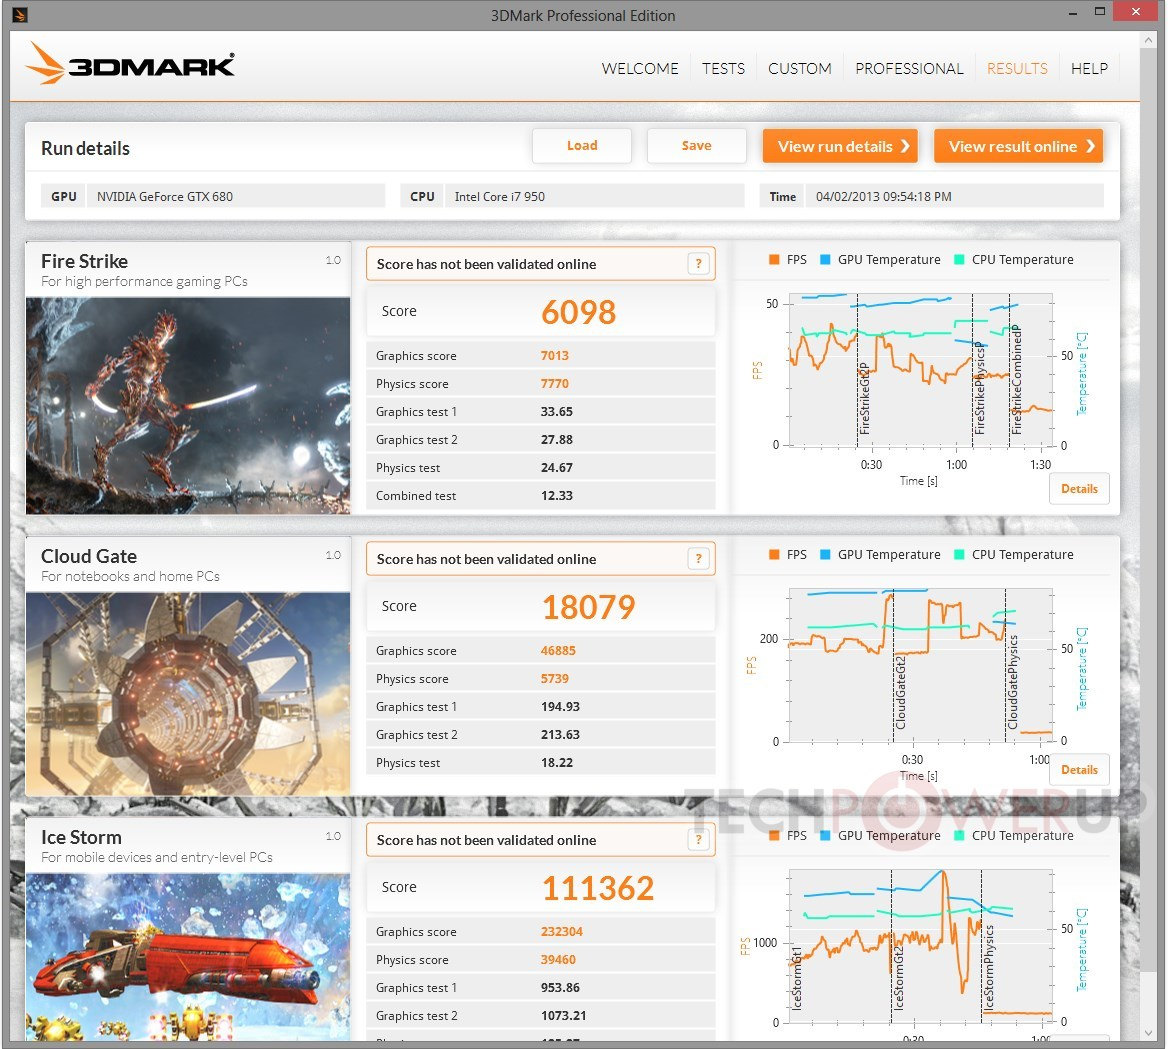
\includegraphics[width=0.7\textwidth]{images/001-3dm2}
	\caption{Подпись рисунка 01}
	\label{img:01:3dm2}
\end{figure}

\begin{figure}[hp]
	\centering
	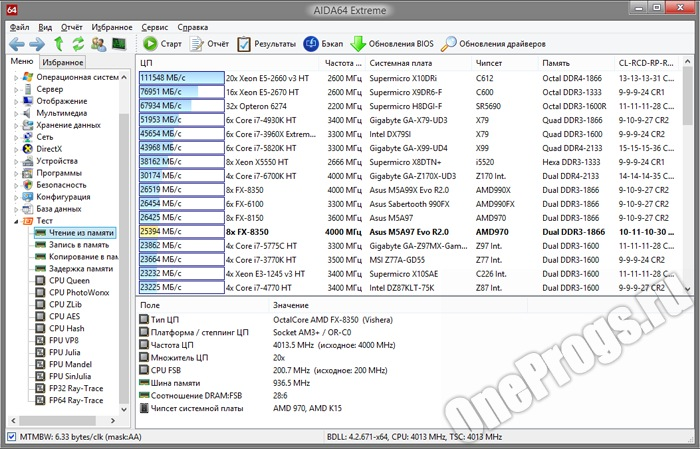
\includegraphics[width=0.7\textwidth]{images/002-AIDA64_scr}
	\caption{Подпись рисунка 02}
	\label{img:01:002-AIDA64_scr}

\end{figure}

\begin{verbatim}

from . import models
import django_filters


class DRYFilter(django_filters.FilterSet):
    name = django_filters.CharFilter(lookup_expr='icontains')
    score = django_filters.RangeFilter()
    rank = django_filters.NumberFilter()
    in_stock = django_filters.BooleanFilter()
    price = django_filters.RangeFilter()

\end{verbatim}

\end{document}